\section{Environment Breadth}
\label{sec:coverage}

\trace contains 1,000 tasks organized into 277
scene grammars across 11 visual domains.  These domains are not reasoning
labels: each groups scenes with related visible inputs, rendering conventions,
and object vocabularies. Figure~\ref{fig:domain-landscape} shows the resulting
distribution without implying that domains are balanced sampling units. The
generated examples in Figure~\ref{fig:domain-montage} illustrate their visual
breadth, while compact construction profiles and a domain-stratified atlas
appear in Appendix~\ref{app:generation} and Appendix~\ref{app:task-atlas}.

\begin{figure*}[t]
  \centering
  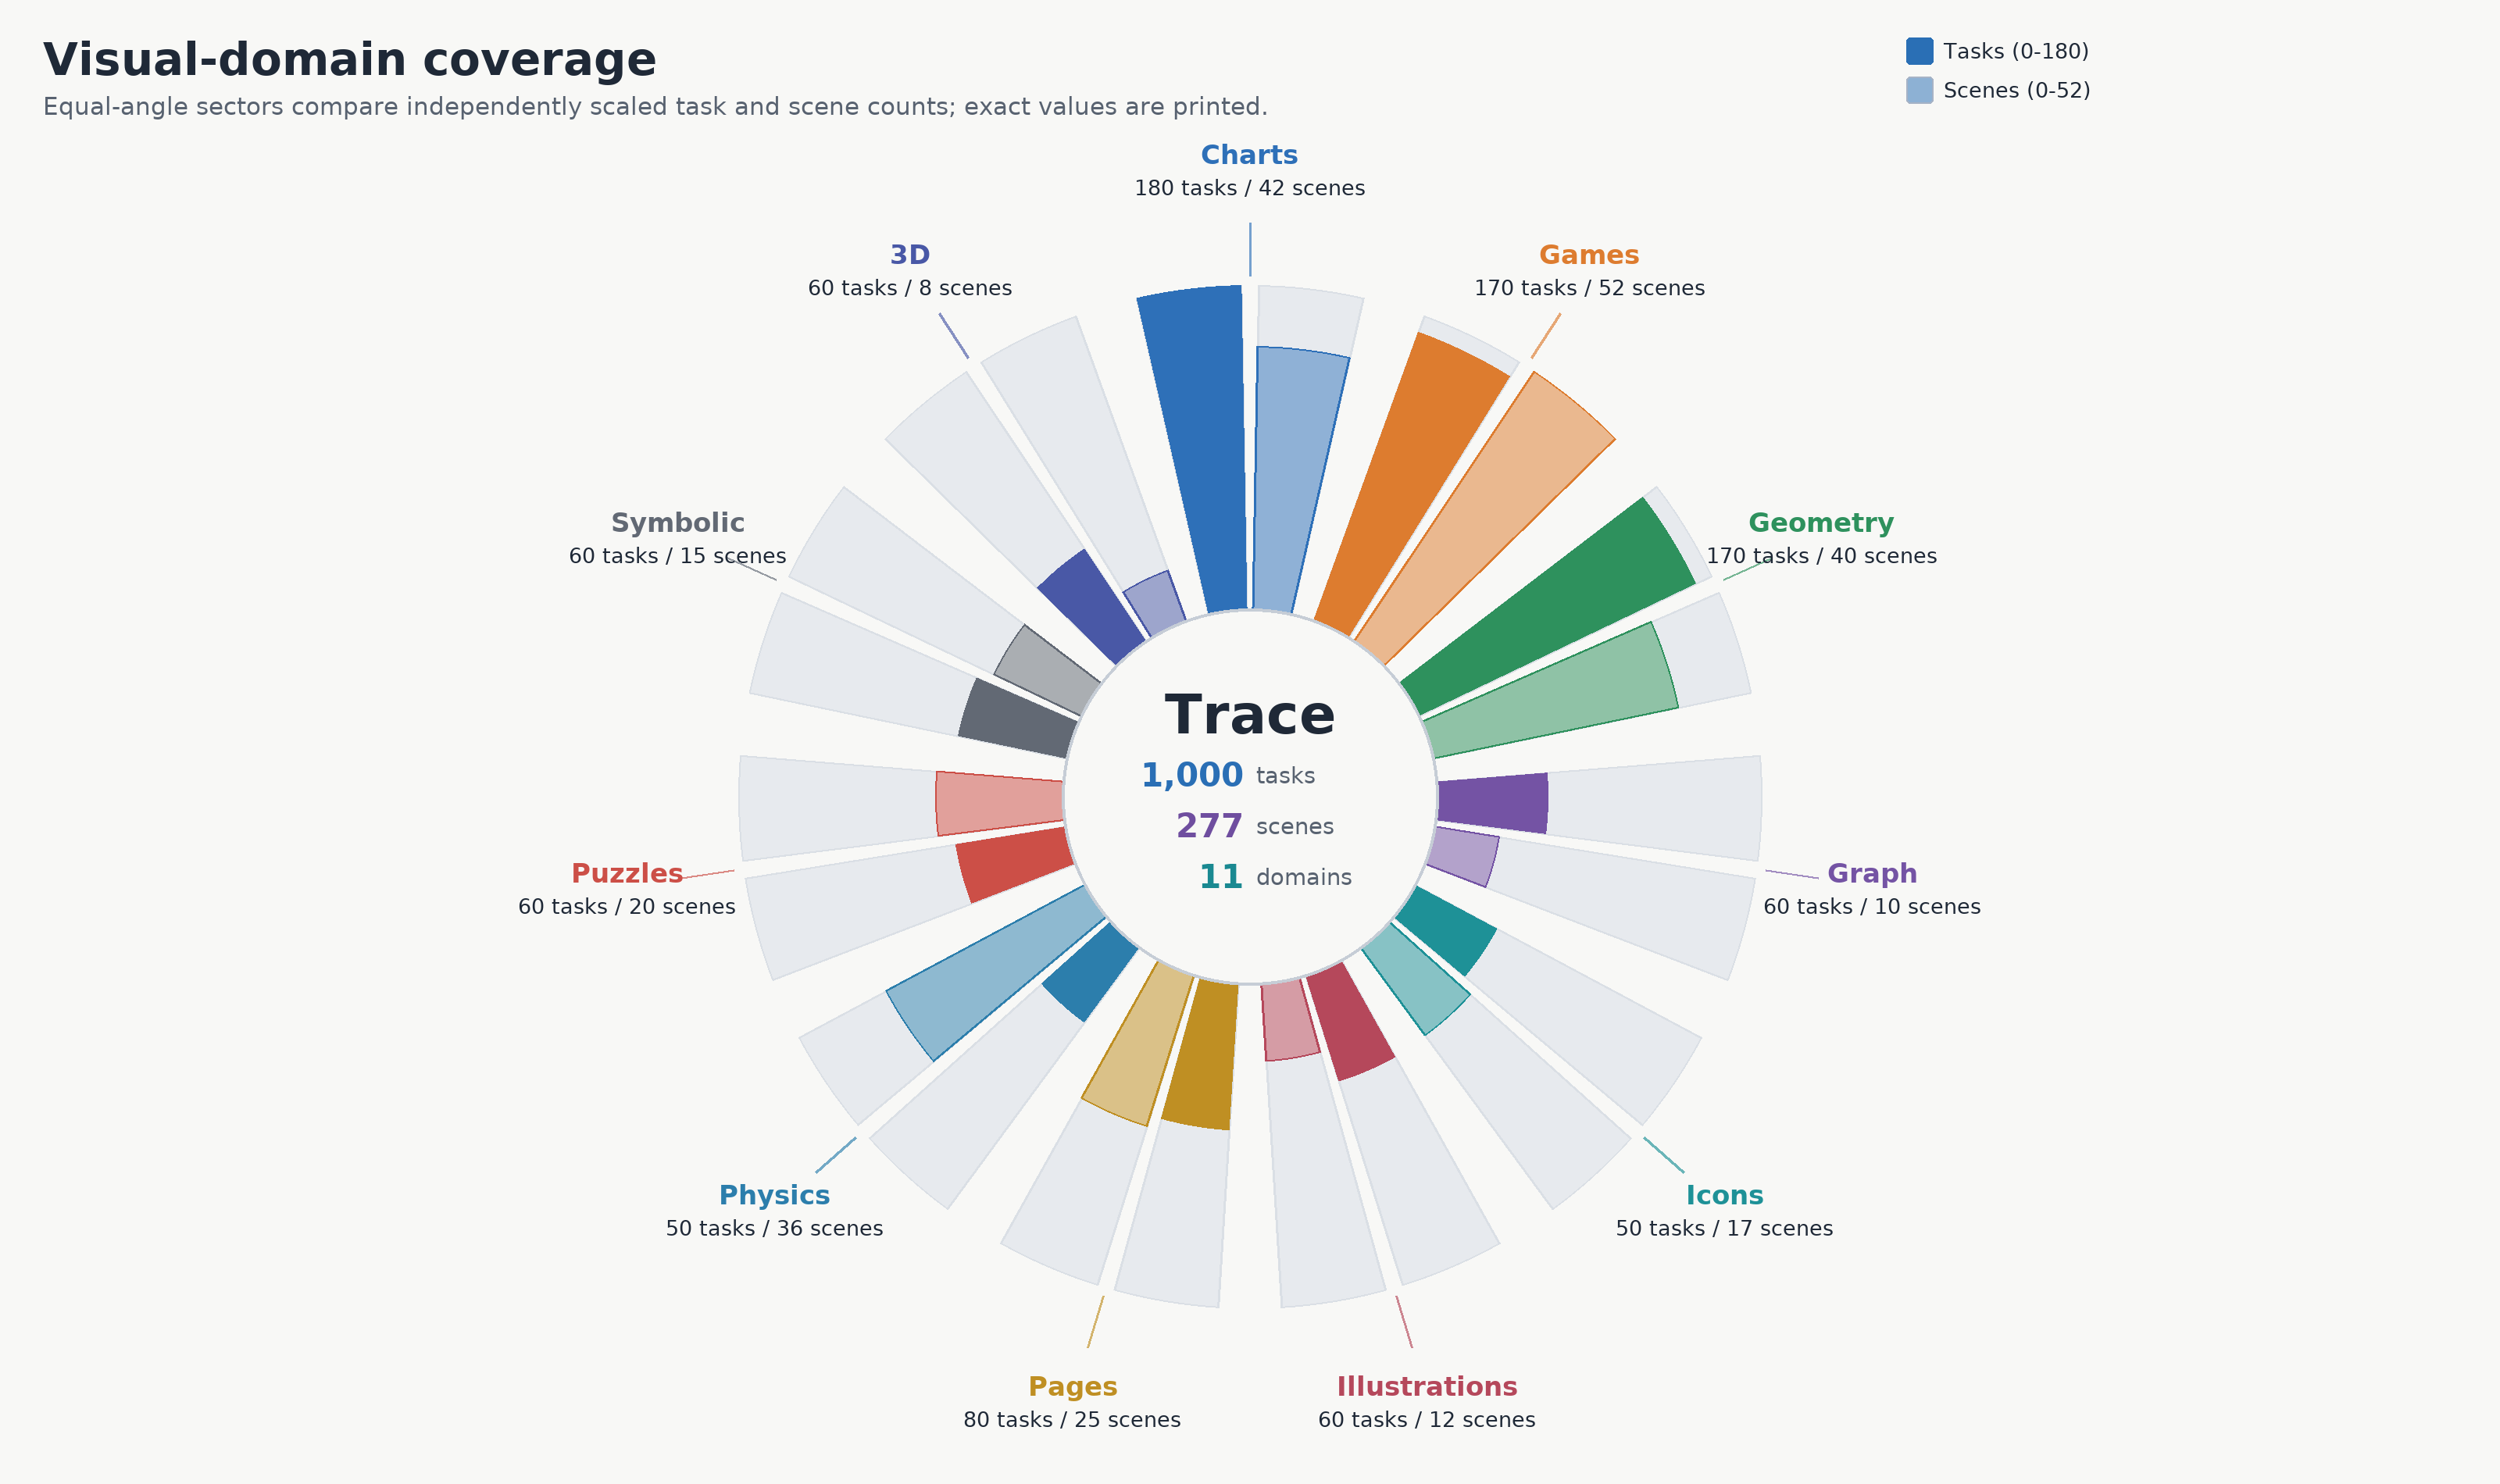
\includegraphics[width=\textwidth]{figures/domain_landscape.png}
  \caption{Scene and task coverage across the 11 visual domains. Each domain
  receives equal angular space. Paired radial bars encode task and scene counts
  on separate scales, with exact counts printed at every sector. Domain totals
  are computed from the complete task set.}
  \label{fig:domain-landscape}
\end{figure*}
\FloatBarrier

Domain counts measure visual breadth but not operational breadth. We therefore
use 13 compositional operation families that cover the active task programs.
Figure~\ref{fig:domain-operation-matrix} summarizes recurring
executable operations across domains. This is an analysis view rather than
another taxonomy level: each task contributes to every selected family that
materially determines its answer. Assignments are derived from the formal task
programs; composed programs may receive multiple assignments, while every task
appears in at least one family. Primitive visual access, output binding, and
annotation construction are excluded; direct retrieval is used only when no
other meaningful operation applies.

\begin{figure*}[t]
  \centering
  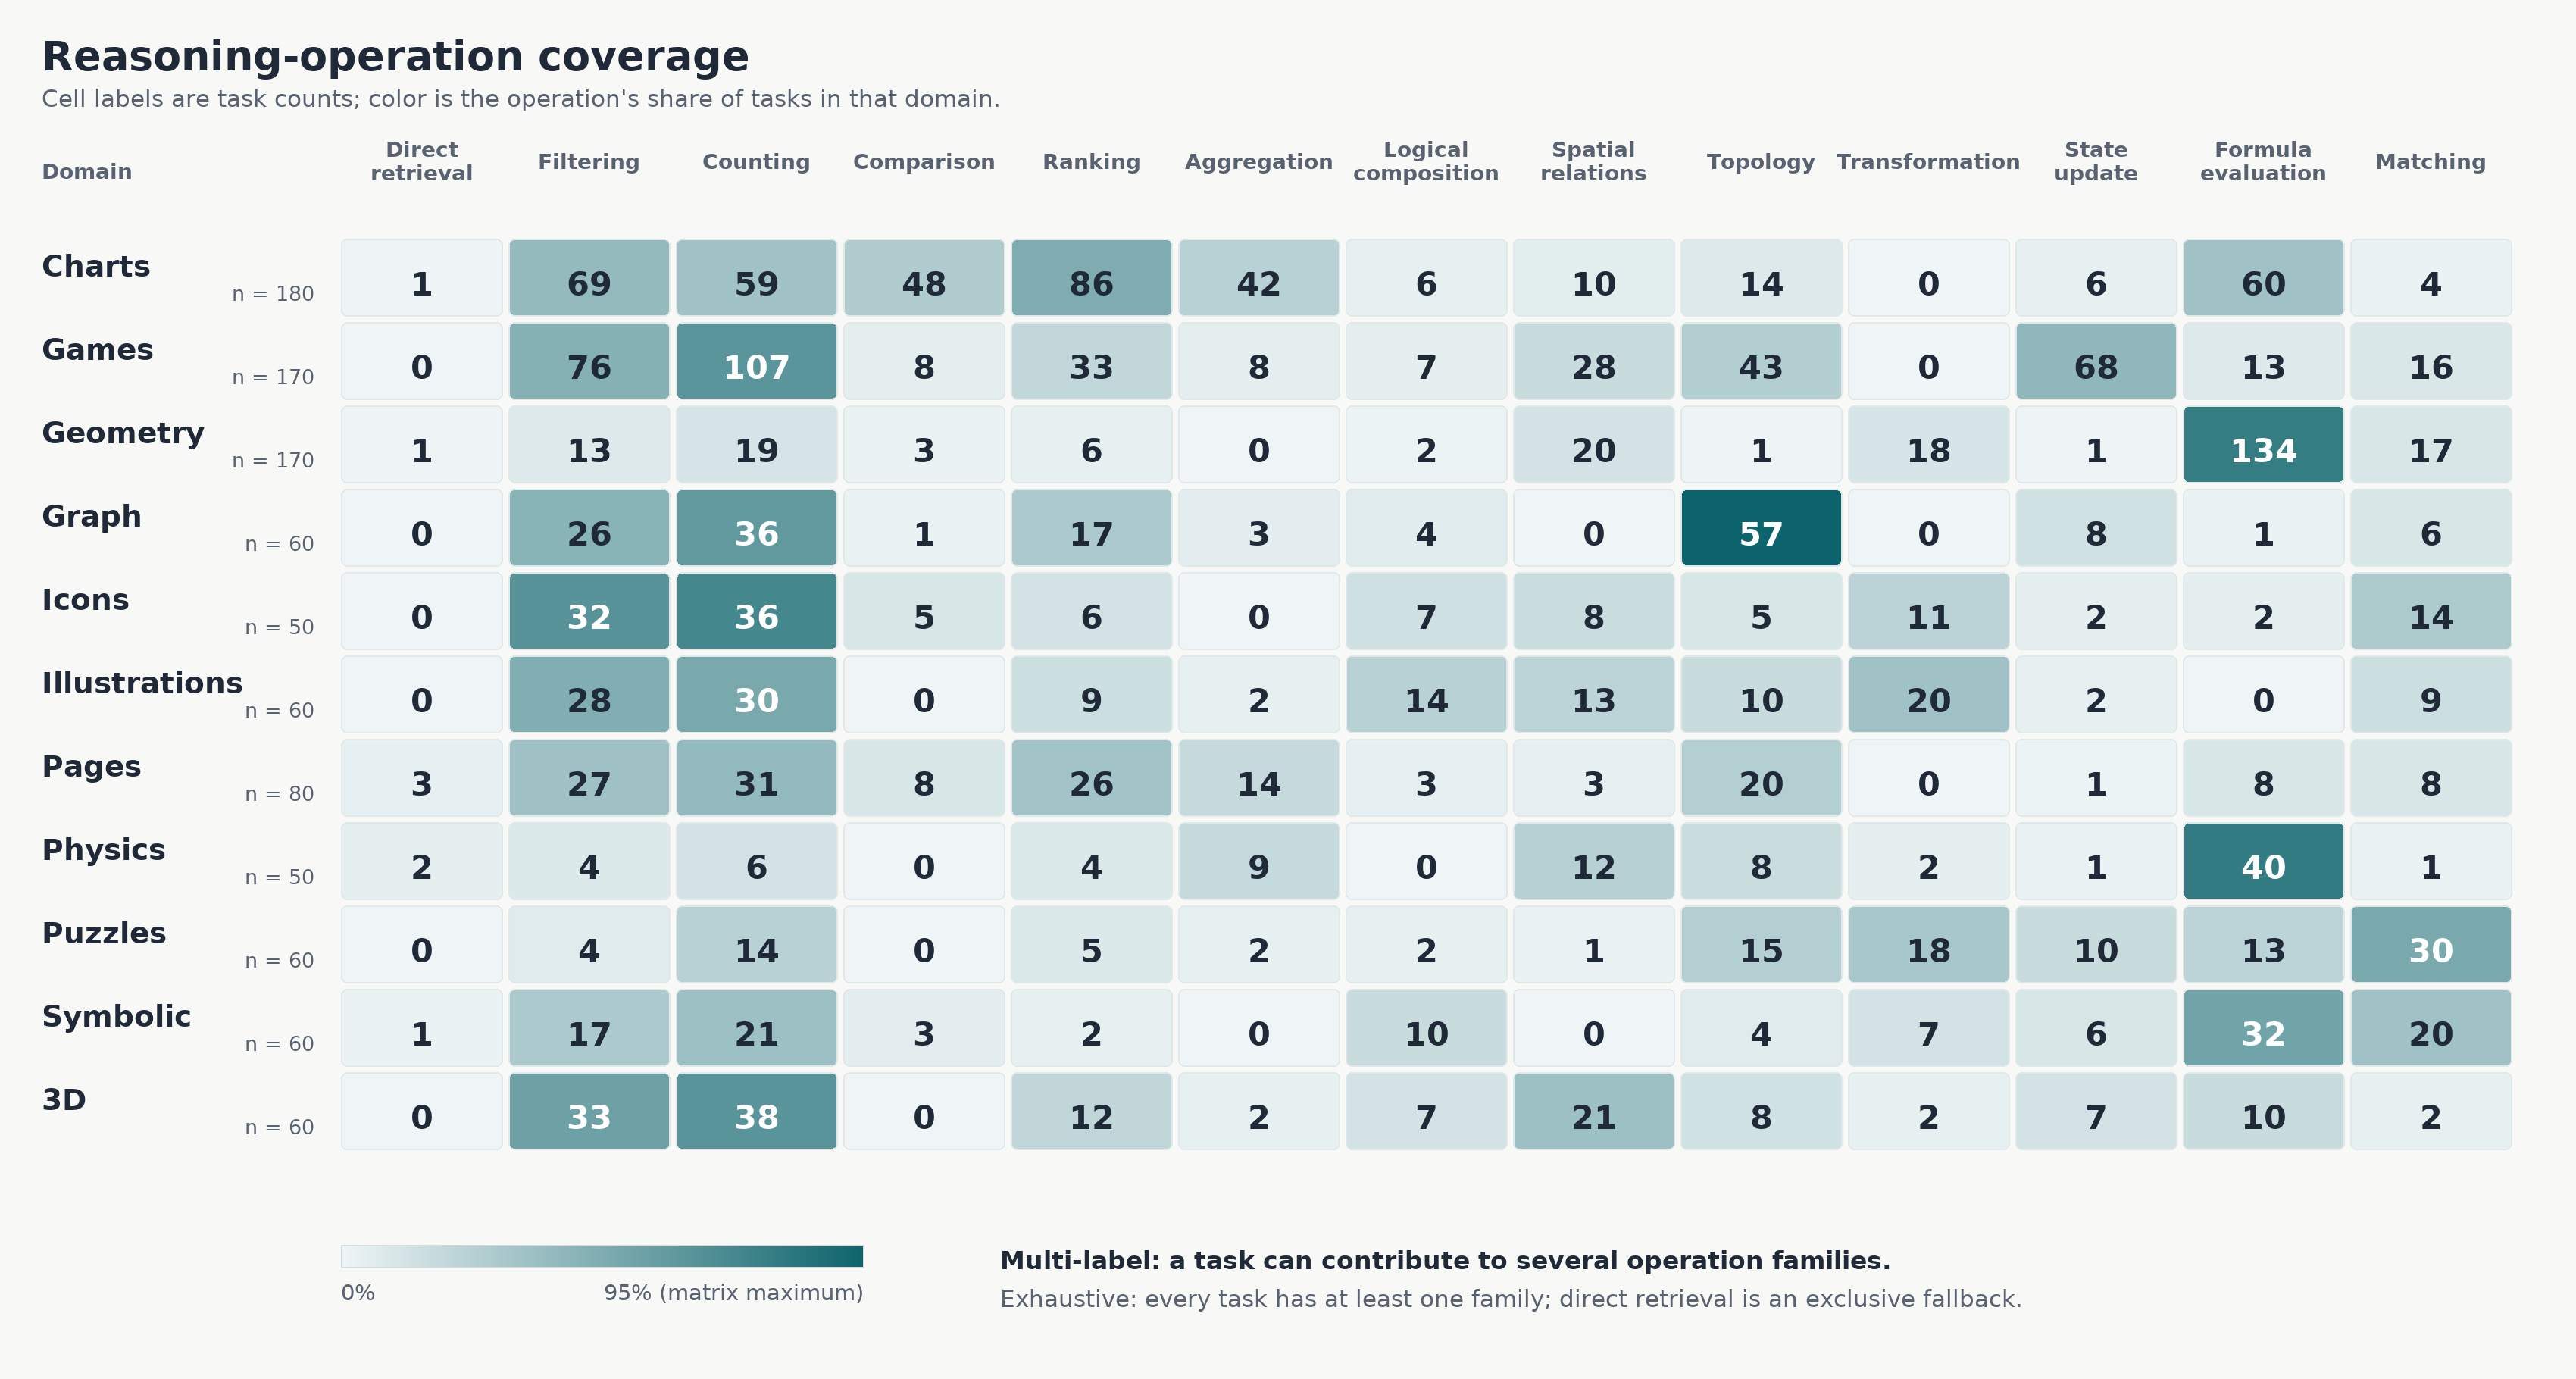
\includegraphics[width=\textwidth]{figures/domain_operation_matrix.png}
  \caption{Cross-domain reasoning-operation coverage. Cell labels are task
  counts, and color encodes the fraction of tasks in that domain. Categories
  are exhaustive and multi-label, so composed programs may occupy several
  columns while every active task appears at least once.}
  \label{fig:domain-operation-matrix}
\end{figure*}

A scene contains a median of three tasks (mean 3.61, range 1--26), reflecting
the policy that scenes are visual grammars rather than fixed-size task
bundles.  The answer interface is also heterogeneous: 547 tasks return
integers, 51 return other numeric values, 192 return visible string labels,
and 210 select rendered options. Thus, 790 tasks use open-form numeric or
string outputs rather than multiple choice. A generated distribution summary
appears in Appendix~\ref{fig:environment-coverage}.

Internal query branches express bounded semantic arguments without inflating
the task count. Of the 1,000 tasks, 317 expose more than one query
branch, for 1,475 branches in total.  Largest versus smallest, above versus
below, or source versus target can therefore vary inside a stable objective
contract while task-level sampling remains the balancing unit. Domain
counts are consequently determined by the number of retained objective
contracts, not by forcing equal numbers of scenes or branches into each
domain.
